\documentclass[a4]{scrartcl}

% \usepackage[ngerman]{babel}
\usepackage[utf8]{inputenc}
\usepackage{mathtools}
\usepackage{amsmath}
\usepackage{amssymb}
\usepackage{geometry}
\usepackage{scrlayer-scrpage}
\pagestyle{scrheadings}
\usepackage{tablefootnote}
\usepackage[dvipsnames]{xcolor}
\usepackage{comment}
\usepackage{enumitem}
% \clearscrheadfoot

\setlength{\parindent}{0em}

\setlength{\parskip}{1.3ex}

\usepackage[onehalfspacing]{setspace}


\clubpenalty = 10000
\widowpenalty = 10000
\displaywidowpenalty = 10000

\usepackage{hyperref}
\hypersetup{
	colorlinks=true,
	linkcolor=black,
	filecolor=black,      
	urlcolor=MidnightBlue,
	citecolor=black
}


\geometry{
	paper=a4paper, % Change to letterpaper for US letter
	top=3cm, % Top margin
	bottom=3cm, % Bottom margin
	left=2cm, % Left margin
	right=3cm, % Right margin
	%showframe, % Uncomment to show how the type block is set on the page
}

\usepackage[backend=biber, maxbibnames=99]{biblatex}
\addbibresource{references.bib}



\usepackage[framemethod=TikZ]{mdframed}

% Style %
\mdfdefinestyle{enviStyle}{
	innertopmargin = 10pt,
	linewidth      = 1pt,
	frametitlerule = true,
	roundcorner    = 2pt%
}


\usepackage{sectsty}
\sectionfont{\color{MidnightBlue}}
\subsectionfont{\color{MidnightBlue}}



\newenvironment{CountingDefinition}[2][]{%
	\ifstrempty{#1}%
	{\mdfsetup{%
			frametitle={{\strut ~}}}
	}%
	{\mdfsetup{%
			frametitle={{\strut ~#1}}}%
	}%
	\mdfsetup{
		nobreak                   = true,
		linecolor                 = MidnightBlue,
		frametitlebackgroundcolor = MidnightBlue!50,
		style                     = enviStyle
	}
	\begin{mdframed}[]\relax%
		\label{#2}}{\end{mdframed}}



\renewcommand{\labelitemi}{$\textcolor{MidnightBlue}{\bullet}$}
\renewcommand{\labelitemii}{$\textcolor{MidnightBlue}{\cdot}$}
\renewcommand{\labelitemiii}{$\textcolor{MidnightBlue}{\diamond}$}
\renewcommand{\labelitemiv}{$\textcolor{MidnightBlue}{\ast}$}





%\ohead{\\
%	Pina Kolling\\
%	piko0011}

\begin{document}
	
	\begin{titlepage}
		\centering
		{\scshape\LARGE Umeå University \par}
		\vspace{1cm}
		{\scshape\Large Managing the Digital Enterprise \par }
		\vspace{1.5cm}
		{\huge\bfseries   {\color{MidnightBlue}Individual Assignment 4} \par}
		\vspace{2cm}
		{\Large\itshape Pina Kolling\par}
		\vfill
		supervised by \par 
		\vspace{1cm}
		Dr. Daniel \textsc{Skog} \par 
		and \par 
		M. Sc. Ramy \textsc{Shenouda} 
		
		\vfill
		
		% Bottom of the page
		{\large \today\par}
	\end{titlepage}
	
	\setcounter{page}{1}
	
	\begin{doublespace}
		\tableofcontents
	\end{doublespace}

	
	\newpage

%The concept of digital transformation is understood differently by different people in both research and practice. Considering the amount of resources that are being invested in strategic digital transformation initiatives, it is of vital importance that managers of digital enterprises have a clear view of what it entails. In particular, it is of high importance that managers understand the extent of change that is involved for the organization. Your task in this assignment is to provide a synthesis of research that a manager of a digital enterprise can use to understand when a change stemming from technology emergence and use should be considered a digital transformation and not. Based on your synthesis, your task is also to provide research-grounded advice on what a manager could expect and plan for when initiating digital transformation in the organization. Specifically, your task is to:












% 1. Value, select and summarize research concepts, perspectives and arguments from at least three of the papers below concerning when a process should be considered to be a digital transformation and not. 
%-------------------------------------------------------------------------------------------
	\section{Definitions of Digital Transformation} \label{sec:Sec1}







%-------------------------------------------------------------------------------------------	
	\subsection{Paper: \textit{Digital doesn't have to be disruptive}} \label{disruptive}
	
	The authors Nathan Furr and Andrew Shipilov described digital transformation in \textit{Digital doesn't have to be disruptive: the best results can come from adaptation rather than reinvention}~\cite{disruptive} as ``adapting an organization's strategy and structure to capture opportunities enabled by digital technology``~\cite[p. 96]{disruptive}.
	The main aspects of digital transformation are listed as automation, virtualization, more targeted product and service customization, more informed decision making and machine-driven recommendations. Those technologies can be applied at almost every company and in almost every step of their processes.~\cite{disruptive}
	
	It can be difficult for companies to create a plan on how to act and execute their digital transformation. But radical replacements are only sometimes necessary -- digital transformation means incremental steps to improve the processes. This includes getting more efficient and user-friendly using digital tools, finding the best way to reach the company's goals through digital tools or to overcome previous challenges.~\cite{disruptive}
	









%-------------------------------------------------------------------------------------------	
\subsection{Paper: \textit{Five myths about digital transformation}} \label{5myths}	
	
	Stephen J. Andriole stated in \textit{Five myths about digital transformation}~\cite{5myths} that the path to digital transformation can be risky, even if it might lead to efficiency, innovation and competitiveness.
	According to the author, companies will fail to implement digital transformation unless it is extremely well planned and executed. There were five myths about digital transformation collected and presented to raise awareness to the risks and dangers of digital transformation. The resulting guidelines from those five myths are summarized in the following.~\cite{5myths}
	\begin{enumerate}
		\item ``Not every company, process, or business model requires digital transformation``~\cite[p. 20]{5myths}
		\item Digital transformation does not necessarily use emerging or disruptive technologies.
		\item If the company is already thriving, the transformation will not have a meaningful impact.
		\item Disruptive transformation does usually not begin with the market leaders.
		\item The executives do not necessarily want to transform digitally.
	\end{enumerate}
	
	










%-------------------------------------------------------------------------------------------	
\subsection{Paper: \textit{IT-enabled business transformation}} \label{venkat}	

In \textit{IT-enabled business transformation: from automation to business scope redefinition}~\cite{venkat} by Nramanujam Venkatraman was stated that IT has a distinctive role in shaping the future's business operations while being a fundamental enabler in creating and maintaining competitiveness.
Five levels of digital transformation were introduced and it was suggested that companies should at first estimate the costs and efforts in comparison to the benefits and then move to higher levels of the transformation. Those levels are summarized in the following.~\cite{venkat}

\begin{description}
	\item[Level 1] Localized Exploitation: 
	
	Deployment of standard IT applications with minimal changes to the business processes.
	
	\item[Level 2] Internal Integration: 
	
	Deployment of IT applications in the entire business process.
	
	\item[Level 3] Business Process Redesign: 
	
	Renewing of processes to improve efficiency with IT applications.
	
	\item[Level 4] Business Network Redesign: 
	
	Execution of digital transformation not only within the organization but with partners or suppliers.
	
	\item[Level 5] Business Scope Redefinition: 
	
	Redefining the market and the company's goals and potentially outsource tasks to third party companies.
	
\end{description}


	
	
	
	
	
	
	
%-------------------------------------------------------------------------------------------	
\subsection{Paper: \textit{Understanding digital transformation}} \label{vial}	
	
Gregory Vial in \textit{Understanding digital transformation: A review and a research agenda}~\cite{vial} stated that digital transformation consists out of 8 building blocks: Digital technologies, disruption, strategic responses, value creation paths, structural changes, organizational barriers and positive and negative outcomes.
Those building blocks and their connection build a framework, that was visualized. This can be seen in Figure \ref{vial_framework}.~\cite{vial}

\begin{figure}[h!]
	\centering
	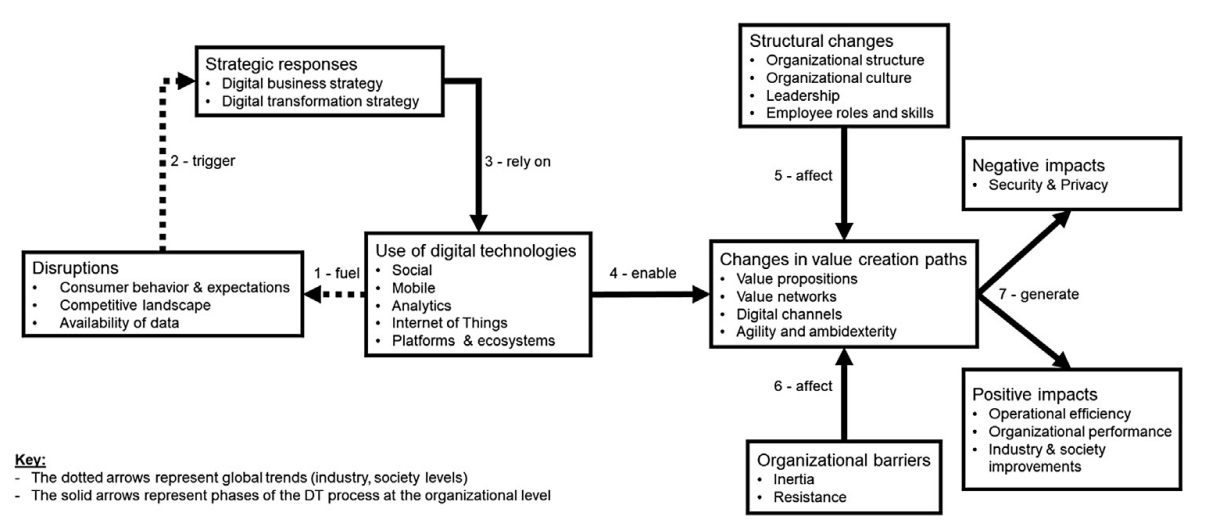
\includegraphics[width=1\textwidth]{images/vial.png}
	\caption{Digital transformation framework \cite{vial}}
	\label{vial_framework}
\end{figure}


The framework shows the process of digital transformation where digital technologies creates disruptions in the global market, triggering global strategic responses from organizations. The organizations then rely on the use of digital technologies. Those technologies enable changes in value creation paths within the organization, which are based on structural changes in the organization and limited by organizational barriers. This results into positive and negative impacts for the organization.~\cite{vial}

% TODO table with different definitions of digital transformation









	





%-------------------------------------------------------------------------------------------	
\subsection{Paper: \textit{Digital Transformation versus IT-Enabled Transformation}} \label{DTOT}	

Lauri Wessel, Abayomi Baiyere, Roxana Ologeanu-Taddei, Jonghyuk Cha and Tina Blegind-Jensen in \textit{Unpacking the difference between digital transformation and IT-enabled organizational transformation}~\cite{DTOT} focus on the difference between digital transformation and IT-enabled transformation. In previous literature, digital transformation and IT-enabled transformation was often examined regarding the strategic significance while emphasizing the similarities of those two concepts. 
In contrast to this, the authors stated that digital transformation can lead to a new organizational identity while IT-enabled organizational transformation is the enhancement of an existing organizational identity.~\cite{DTOT}
	









\begin{comment}

%-------------------------------------------------------------------------------------------	
\subsection{Examples: Digital transformation or not?} \label{DTornotDT}

In the following table, example processes are listed and categorized into \textit{Digital transformation or not}, given the definition from the previously described literature.
	
	\begin{table}[h]
		\centering
		\begin{tabular}{|p{11cm}|c|c|c|c|c|}
			\hline
			\textbf{Processes} & \cite{5myths} & \cite{disruptive} & \cite{venkat} & \cite{vial} & \cite{DTOT} \\
			\hline
			\hline
			Introducing a new software to organize internal processes & Yes & & & & \\
			\hline
			Automating order processing and fulfillment & Yes & & & & \\
			\hline
			Restructuring the company's organizational hierarchy & No & & & & \\
			\hline
			Upgrading the network infrastructure for better connectivity & Yes & & & & \\
			\hline
			Developing a mobile app for customer interactions & Yes & & & & \\
			\hline
			Adopting data analytics for decision-making & Yes & & & & \\
			\hline
			Migrating to a paperless document management system & Yes & & & & \\
			\hline
			Outsourcing IT services to a third-party provider & No & & & & \\
			\hline
			Implementing a remote work policy and tools & Yes & & & & \\
			\hline
			Enhancing cybersecurity measures & Yes & & & & \\
			\hline
			Automating the employee onboarding process & Yes & & & & \\
			\hline
		\end{tabular}
	\end{table}
	
\end{comment}
	









% 2. Analyze and synthesize the concepts, perspectives and arguments to individually argue for 3-4 key characteristics that can be used to determine whether a process should be considered to be a digital transformation and not. 
%-------------------------------------------------------------------------------------------
\section{Section 2} \label{sec:Sec2}

In the following, the key attributes for the definition of digital transformation from each of the in Section \ref{sec:Sec1} described papers are listed.





\begin{minipage}{0.5\linewidth}		
	
		\begin{CountingDefinition}[Key attributes~\cite{5myths}]{def:5myths}
		
			\textit{Five myths about digital transformation}~\cite{5myths}
			
			\begin{itemize}[noitemsep,topsep=0pt]
				\item Not every company or process needs digital transformation
				\item Radical replacements are often not necessary (no disruptiveness)
			\end{itemize}
		
		
		\end{CountingDefinition}	
	

	
\end{minipage}	\begin{minipage}{0.5\linewidth}


	\begin{CountingDefinition}[Key attributes~\cite{disruptive}]{def:disruptive}
	
		\textit{Digital doesn't have to be disruptive}~\cite{disruptive}
		
		\begin{itemize}[noitemsep,topsep=0pt]
			\item Incremental steps to improve processes
			\item Radical replacements are often not necessary (no disruptiveness)
		\end{itemize}
	
	
	\end{CountingDefinition}
	


\end{minipage}






\begin{CountingDefinition}[Key attributes~\cite{venkat}]{def:venkat}
	
		\textit{IT-enabled business transformation}~\cite{venkat}
		
		\begin{itemize}[noitemsep,topsep=0pt]
			\item Incremental steps to improve processes presented as levels (no disruptiveness)
		\end{itemize}


\end{CountingDefinition}





\begin{minipage}{0.5\linewidth}			
	
	\begin{CountingDefinition}[Key attributes~\cite{vial}]{def:vial}
		
		\textit{Understanding digital transformation}~\cite{vial}
		
		\begin{itemize}[noitemsep,topsep=0pt]
			\item Changes are responses to disruption that happen through the use of digital technologies (disruptiveness)
		\end{itemize}

		
	\end{CountingDefinition}
	
\end{minipage}	\begin{minipage}{0.5\linewidth}
	
	\begin{CountingDefinition}[Key attributes~\cite{DTOT}]{def:DTOT}
		
		\textit{Digital vs. IT-enabled transformation}~\cite{DTOT}
		
		\begin{itemize}[noitemsep,topsep=0pt]
			\item Digital transformation can lead to a new organizational identity (disruptiveness)
		\end{itemize}

		
	\end{CountingDefinition}
	
\end{minipage}

\ 

One key aspect that was emphasized in the literature, is the aspect of realizing digital transformation incremental and step by step \cite{5myths, disruptive, venkat}.
This is reasoned by several advantages:

\begin{itemize}
	
	
	\item \textbf{Risk reduction:}
	
	Digital transformation can be complex and risky. Incrementally introducing changes allows organizations to identify and address issues one by one. \cite{5myths}
	
	
	\item \textbf{Resource Management:}
	
	Smaller changes can help managing the budget and employees. TODO source!
	
	\item \textbf{Acceptance:} 
	
	Employees are more likely to accept changes when it happens gradually and smaller steps can create more opportunities for training and adaptation. \cite{acceptance, wiwi}
	
	%4. **Testing and Learning:** Step-by-step transformations provide a learning curve for the organization. Each phase allows for testing, refinement, and learning from mistakes, ultimately leading to better outcomes in subsequent phases.
	
	%5. **Flexibility:** Digital technologies and business environments are constantly evolving. Smaller steps allow organizations to pivot and adapt to changing circumstances more easily, ensuring that they remain agile and responsive.
	
	%6. **Measurable Progress:** Incremental transformations make it easier to measure and demonstrate progress, which is essential for tracking the return on investment and securing stakeholder buy-in.
	
	%7. **Customer Experience:** By taking smaller steps, organizations can maintain a focus on customer needs and feedback, continually improving their digital offerings based on real-world use and customer preferences.
	
	%8. **Preserving Core Functions:** Smaller, phased implementations can help ensure that core business functions are not disrupted by attempting too much change at once.
	
	%9. **Cultural Alignment:** Building a culture of digital innovation and adaptation often requires time. Smaller steps allow employees to gradually align with the organization's digital goals and values.
	
	%10. **Easier Troubleshooting:** When issues arise during digital transformation, they can be addressed more effectively in smaller phases, preventing larger-scale failures.
	
	
\end{itemize}






%In summary, a step-by-step approach to digital transformation allows organizations to manage risks, engage employees, adapt to changing circumstances, and ensure that the transformation aligns with both the company's goals and customer expectations. This approach not only reduces the challenges associated with digital transformation but also increases the likelihood of long-term success.


%------------------------------------------------------------------------------------------------------------

%In the context of digital transformation, disruption refers to a significant and often abrupt change or transformation in the way traditional industries, businesses, or processes operate due to the adoption and integration of digital technologies, strategies, and innovations. This disruption typically results in a fundamental shift in the status quo, business models, and customer expectations, leading to a new competitive landscape.

%Key characteristics of disruption in digital transformation include:

%1. **Technological Innovation:** Disruption is often driven by the introduction of new digital technologies or innovative applications of existing technologies that challenge established norms and practices.

%2. **Market Transformation:** It reshapes markets and industries, often leading to the displacement of traditional players, the emergence of new leaders, and the creation of new business opportunities.

%3. **Customer-Centric Focus:** Disruption in digital transformation is frequently centered around meeting evolving customer needs and expectations, often with more personalized and convenient solutions.

%4. **Rapid Change:** Digital disruption can occur swiftly, catching traditional organizations off guard and necessitating quick adaptations to stay competitive.

%5. **Efficiency and Productivity Gains:** It can result in improved operational efficiency, reduced costs, and increased productivity through automation and data-driven decision-making.

%Examples of digital disruption include the rise of e-commerce, which transformed the retail industry, and the adoption of ride-sharing apps, which disrupted the taxi and transportation sector. In essence, digital disruption involves a radical shift that challenges existing business models and necessitates a reevaluation of strategies and practices to thrive in the digital age.
















% 3. Use the 3-4 key characteristics to explain what scope and scale of change a manager should expect and plan for when initiating a digital transformation initiative and the most important things a manager needs to think about to manage it successfully
%-------------------------------------------------------------------------------------------
\section{Section 3} \label{sec:Sec3}

\begin{CountingDefinition}[Definitions]{def:defdef}
	

		
		Text

	
\end{CountingDefinition}













%-------------------------------------------------------------------------------------------
	
	\newpage
	\addcontentsline{toc}{section}{References}
	\begin{spacing}{0.9}
		\printbibliography
	\end{spacing}


	
	
	
	
	
	
\end{document}